\subsection{相切在作图中的应用}\label{subsec:czjh2-7-15}

运动场上的跑道和有些凸轮的轮廓线(图 \ref{fig:czjh2-7-58})等,是由线段和圆弧或几段圆弧平滑地连接起来的。

\begin{figure}[htbp]
    \centering
    \begin{minipage}[b]{6cm}
        \centering
        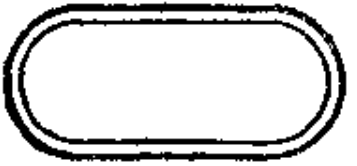
\includegraphics[width=5.5cm]{../pic/czjh2-ch7-58-1.png}
    \end{minipage}
    \qquad
    \begin{minipage}[b]{4cm}
        \centering
        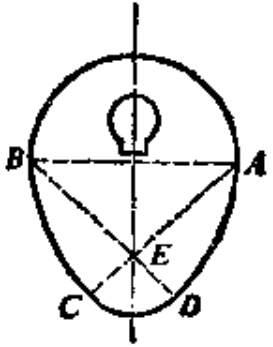
\includegraphics[width=3.5cm]{../pic/czjh2-ch7-58-2.png}
    \end{minipage}
    \caption{}\label{fig:czjh2-7-58}
\end{figure}

线段所在的直线(圆弧所在的圆)与圆弧所在的圆相切于某一点,并且在切点的两侧,
就说线段(圆弧)和圆弧在这一点\zhongdian{连接}。
如图 \ref{fig:czjh2-7-59} 中,线段 $AB$ 和弧 $\yuanhu{AC}$ 在点 $A$ 连接,
图 \ref{fig:czjh2-7-60} 中, $\yuanhu{AB}$ 和 $\yuanhu{AC}$ 在点 $A$ 连接。

\begin{figure}[htbp]
    \centering
    \begin{minipage}[b]{5cm}
        \centering
        \begin{tikzpicture}
    \pgfmathsetmacro{\R}{1.5}

    \tkzDefPoints{0/0/O}
    \tkzDefPoint(270:\R){A}
    \tkzDefShiftPoint[A](2,0){B}
    \tkzDefShiftPoint[A](-2,0){B'}
    \tkzDefPoint(140:\R){C}

    \tkzDrawPoint(O)
    \tkzDrawArc[dashed](O,A)(C)
    \tkzDrawArc[thick](O,C)(A)
    \tkzDrawSegment[red](O,C)
    \tkzLabelSegment[above](O,C){$R$}
    \tkzDrawSegment[dashed](O,A)
    \tkzLabelPoints[right](O)
    \tkzLabelPoints[left](C)

    \tkzDrawSegment[thick](A,B)
    \tkzDrawSegment[dashed](A,B')
    \tkzLabelSegment[pos=1, left](B,B'){$l$}
    \tkzLabelPoints[below](A)
    \tkzLabelPoints[right](B)
\end{tikzpicture}


        \caption*{} % 与下面的图水平对齐
        \caption{}\label{fig:czjh2-7-59}
    \end{minipage}
    \qquad
    \begin{minipage}[b]{10.5cm}
        \centering
        \begin{minipage}[b]{5.6cm}
            \centering
            \begin{tikzpicture}
    \pgfmathsetmacro{\R}{1.5}
    \pgfmathsetmacro{\r}{0.8}

    \tkzDefPoints{0/0/O_1, \R+\r/0/O_2, \R/0/A}
    \tkzDefPoint(70:\R){B}
    \tkzDefPoint(60:\R){M}
    \tkzDefShiftPoint[O_2](270:\r){C}
    \tkzDefShiftPoint[O_2](60:\r){N}
    \tkzDefLine[perpendicular=through A, normed](O_1,O_2)  \tkzGetPoint{a}

    \tkzDrawPoint(O_1)
    \tkzDrawArc[thick](O_1,A)(B)
    \tkzDrawArc[dashed](O_1,B)(A)
    \tkzDrawSegment[red](O_1,M)
    \tkzLabelSegment[pos=.7, below, xshift=.3em](O_1,M){$R_1$}
    \tkzLabelPoints[below](O_1)
    \tkzLabelPoints[above](B)

    \tkzDrawPoint(O_2)
    \tkzDrawArc[thick](O_2,A)(C)
    \tkzDrawArc[dashed](O_2,C)(A)
    \tkzDrawSegment[red](O_2,N)
    \tkzLabelSegment[pos=.8, below, xshift=.3em](O_2,N){$R_2$}
    \tkzLabelPoints[below](O_2)
    \tkzLabelPoints[below](C)

    \tkzDrawLine[dashed, add=.8 and .5](O_1,O_2)
    \tkzDrawLine[dashed, add=2 and 1](A,a)
    \tkzLabelPoints[below, xshift=-1em](A)
\end{tikzpicture}


            \caption*{甲}
        \end{minipage}
        \begin{minipage}[b]{4cm}
            \centering
            \begin{tikzpicture}
    \pgfmathsetmacro{\R}{1.5}
    \pgfmathsetmacro{\r}{0.9}

    \tkzDefPoints{0/0/O_1, \R-\r/0/O_2, \R/0/A}
    \tkzDefPoint(270:\R){B}
    \tkzDefPoint(80:\R){M}
    \tkzDefShiftPoint[O_2](70:\r){C}
    \tkzDefShiftPoint[O_2](60:\r){N}
    \tkzDefLine[perpendicular=through A, normed](O_1,O_2)  \tkzGetPoint{a}

    \tkzDrawPoint(O_1)
    \tkzDrawArc[thick](O_1,B)(A)
    \tkzDrawArc[dashed](O_1,A)(B)
    \tkzDrawSegment[red](O_1,M)
    \tkzLabelSegment[pos=.7, left](O_1,M){$R_1$}
    \tkzLabelPoints[below](O_1)
    \tkzLabelPoints[below](B)

    \tkzDrawPoint(O_2)
    \tkzDrawArc[thick](O_2,A)(C)
    \tkzDrawArc[dashed](O_2,C)(A)
    \tkzDrawSegment[red](O_2,N)
    \tkzLabelSegment[pos=.7, below, xshift=.3em](O_2,N){$R_2$}
    \tkzLabelPoints[below](O_2)
    \tkzLabelPoints[above](C)

    \tkzDrawLine[dashed, add=1.2 and .2](O_1,A)
    \tkzDrawLine[dashed, add=2 and 1](A,a)
    \tkzLabelPoints[below, xshift=1em](A)
\end{tikzpicture}


            \caption*{乙}
        \end{minipage}
        \caption{}\label{fig:czjh2-7-60}
    \end{minipage}
\end{figure}

图 \ref{fig:czjh2-7-60} 甲中, $\yuan\,O_1$ 和 $\yuan\,O_2$ 外切于点 $A$,
我们称在连心线 $O_1O_2$ 两旁的 $\yuanhu{AB}$ 和 $\yuanhu{AC}$ 在点 $A$ \zhongdian{外连接}。
图 \ref{fig:czjh2-7-60} 乙中, $\yuan\,O_1$ 和 $\yuan\,O_2$ 内切于点 $A$,
我们称在连心线 $O_1O_2$ 两旁的 $\yuanhu{AB}$ 和 $\yuanhu{AC}$ 在点 $A$ \zhongdian{内连接}。

由连接的定义可知,在图 \ref{fig:czjh2-7-60} 中, $\yuanhu{AB}$ 和 $\yuanhu{AC}$ 在点 $A$ 连接,
就是 $\yuan\,O_1$ 和 $\yuan\,O_2$ 在点 $A$ 相切, 因此点 $A$ 一定在连心线 $O_1O_2$ 上。
利用这个关系,可画圆弧与圆弧在某一点连接。


\liti 已知:如图 \ref{fig:czjh2-7-61}, $\yuanhu{AB}$ 的半径为 $R_1$, 圆心为 $O_1$, 线段 $R_2$。

\begin{wrapfigure}[8]{r}{6cm}
    \centering
    \begin{tikzpicture}
    \pgfmathsetmacro{\R}{1.5}
    \pgfmathsetmacro{\r}{0.9}

    \begin{scope}[xshift=2cm, yshift=1.6cm]
        \tkzDefPoints{0/0/a1, \r/0/a2}
        \tkzDrawSegments[xianduan={below=0pt}](a1,a2)
        \tkzLabelSegment[above](a1,a2){$R_2$}
    \end{scope}

    \tkzDefPoints{0/0/O_1, \R/0/A}
    \tkzDefPoint(120:\R){B}
    \tkzDefPoint(60:\R){M}

    \tkzDrawPoint(O_1)
    \tkzDrawArc[thick](O_1,A)(B)
    \tkzDrawSegment[red](O_1,M)
    \tkzLabelSegment[pos=.7, below, xshift=.3em](O_1,M){$R_1$}
    \tkzLabelPoints[below](O_1)
    \tkzLabelPoints[below left](A)
    \tkzLabelPoints[above](B)

    % 1
    \tkzDefPoints{\R+\r/0/O_2}
    \tkzDrawSegment(O_1, O_2)
    \tkzDrawPoint(O_2)
    \tkzLabelPoints[below](O_2)

    % 2
    \tkzDefShiftPoint[O_2](320:\r){C}
    \tkzDrawArc[thick](O_2,A)(C)
    \tkzLabelPoints[below](C)
\end{tikzpicture}


    \caption{}\label{fig:czjh2-7-61}
\end{wrapfigure}

求作:半径为 $R_2$ 的 $\yuanhu{AC}$, 使 $\yuanhu{AC}$ 与 $\yuanhu{AB}$ 在点 $A$ 外连接。

分析: 要作 $\yuanhu{AC}$ 与 $\yuanhu{AB}$ 外连接,
就是要作 $\yuanhu{AC}$ 和 $\yuanhu{AB}$ 所在的圆在点 $A$ 外切。
因此 $\yuanhu{AC}$ 所在的圆的圆心 $O_2$ 一定在 $O_1A$ 的延长线上,
并且 $O_1O_2 = R_1 + R_2$。

\zuofa 1. 连结 $O_1A$, 并延长到点 $O_2$, 使 $O_1O_2 = R_1 + R_2$。

2. 以 $O_2$ 为圆心, $R_2$ 为半径作 $\yuanhu{AC}$, 使 $\yuanhu{AC}$ 与 $\yuanhu{AB}$ 在 $O_1O_2$ 的两侧。

$\yuanhu{AC}$ 就是所求的弧。

证明略。

% \begin{figure}[htbp]
%     \centering
%     % \begin{minipage}[b]{7cm}
%     %     \centering
%     %     \begin{tikzpicture}
    \pgfmathsetmacro{\R}{1.5}
    \pgfmathsetmacro{\r}{0.9}

    \begin{scope}[xshift=2cm, yshift=1.6cm]
        \tkzDefPoints{0/0/a1, \r/0/a2}
        \tkzDrawSegments[xianduan={below=0pt}](a1,a2)
        \tkzLabelSegment[above](a1,a2){$R_2$}
    \end{scope}

    \tkzDefPoints{0/0/O_1, \R/0/A}
    \tkzDefPoint(120:\R){B}
    \tkzDefPoint(60:\R){M}

    \tkzDrawPoint(O_1)
    \tkzDrawArc[thick](O_1,A)(B)
    \tkzDrawSegment[red](O_1,M)
    \tkzLabelSegment[pos=.7, below, xshift=.3em](O_1,M){$R_1$}
    \tkzLabelPoints[below](O_1)
    \tkzLabelPoints[below left](A)
    \tkzLabelPoints[above](B)

    % 1
    \tkzDefPoints{\R+\r/0/O_2}
    \tkzDrawSegment(O_1, O_2)
    \tkzDrawPoint(O_2)
    \tkzLabelPoints[below](O_2)

    % 2
    \tkzDefShiftPoint[O_2](320:\r){C}
    \tkzDrawArc[thick](O_2,A)(C)
    \tkzLabelPoints[below](C)
\end{tikzpicture}


%     %     \caption{}\label{fig:czjh2-7-61}
%     % \end{minipage}
%     \qquad
%     \begin{minipage}[b]{7cm}
%         \centering
%         \begin{tikzpicture}
    % 1
    \tkzDefPoints{0/0/F, 0/3/E}
    \tkzDrawSegment(E,F)
    \tkzLabelPoints[above](E)
    \tkzLabelPoints[below](F)

    \tkzDefTriangle[equilateral](E,F)  \tkzGetPoint{C}
    \tkzDefTriangle[equilateral](F,E)  \tkzGetPoint{D}
    \tkzDrawPolygon(E,F,C)
    \tkzDrawPolygon(E,F,D)
    \tkzLabelPoints[right](C)
    \tkzLabelPoints[left](D)

    % 2
    \tkzDefMidPoint(C,F)  \tkzGetPoint{K}
    \tkzDefMidPoint(C,E)  \tkzGetPoint{L}
    \tkzInterLL(E,K)(F,L)  \tkzGetPoint{O_1}
    \tkzDrawSegments(E,K  F,L)
    \tkzLabelPoints[below right](K)
    \tkzLabelPoints[above right](L)
    \tkzLabelPoints[left, yshift=.5em](O_1)

    % 3
    \tkzDefMidPoint(D,F)  \tkzGetPoint{N}
    \tkzDefMidPoint(D,E)  \tkzGetPoint{M}
    \tkzInterLL(E,N)(F,M)  \tkzGetPoint{O_2}
    \tkzDrawSegments(E,N  F,M)
    \tkzLabelPoints[below left](N)
    \tkzLabelPoints[above left](M)
    \tkzLabelPoints[right, yshift=.5em](O_2)

    % 4
    \tkzDrawSegment(C,D)
    \tkzCalcLength(O_1,K)  \tkzGetLength{rOK}
    \tkzInterLC[R](C,D)(O_1,\rOK)  \tkzGetFirstPoint{A}
    \tkzInterLC[R](C,D)(O_2,\rOK)  \tkzGetSecondPoint{A'}
    \tkzDrawArc[R with nodes](O_1,\rOK)(K,L)
    \tkzDrawArc[R with nodes](O_2,\rOK)(M,N)
    \tkzLabelPoints[left, yshift=.5em](A)
    \tkzLabelPoints[right=-.2em, yshift=.5em](A')

    % 5
    \tkzCalcLength(E,K)  \tkzGetLength{rEK}
    \tkzInterLC[R](E,F)(F,\rEK)  \tkzGetFirstPoint{B}
    \tkzInterLC[R](E,F)(E,\rEK)  \tkzGetSecondPoint{B'}
    \tkzDrawArc[R with nodes](E,\rEK)(N,K)
    \tkzDrawArc[R with nodes](F,\rEK)(L,M)
    \tkzLabelPoints[below, xshift=-.5em](B)
    \tkzLabelPoints[above, xshift=.5em](B')
\end{tikzpicture}


%         \caption{}\label{fig:czjh2-7-62}
%     \end{minipage}
% \end{figure}


\liti 用圆弧连接,画椭圆的近似图形。

\zuofa 1. 任作一线段 $EF$。 以 $EF$ 为公共边作等边三角形 $CEF$ 和 $DEF$ (图 \ref{fig:czjh2-7-62})。

2. 作 $\triangle CEF$ 的中线 $EK$、$FL$, 相交于点 $O_1$。

3. 作 $\triangle DEF$ 的中线 $EN$、$FM$, 相交于点 $O_2$。

4. 分别以 $O_1$、$O_2$ 为圆心, 以 $O_1K$ 为半径作 $\yuanhu{KAL}$、 $\yuanhu{MA'N}$。

5. 分别以 $E$、$F$ 为圆心, 以 $EK$ 为半径作 $\yuanhu{NB'K}$、 $\yuanhu{MBL}$。

\begin{figure}[htbp]
    \centering
    \begin{minipage}[b]{7cm}
        \centering
        \begin{tikzpicture}
    % 1
    \tkzDefPoints{0/0/F, 0/3/E}
    \tkzDrawSegment(E,F)
    \tkzLabelPoints[above](E)
    \tkzLabelPoints[below](F)

    \tkzDefTriangle[equilateral](E,F)  \tkzGetPoint{C}
    \tkzDefTriangle[equilateral](F,E)  \tkzGetPoint{D}
    \tkzDrawPolygon(E,F,C)
    \tkzDrawPolygon(E,F,D)
    \tkzLabelPoints[right](C)
    \tkzLabelPoints[left](D)

    % 2
    \tkzDefMidPoint(C,F)  \tkzGetPoint{K}
    \tkzDefMidPoint(C,E)  \tkzGetPoint{L}
    \tkzInterLL(E,K)(F,L)  \tkzGetPoint{O_1}
    \tkzDrawSegments(E,K  F,L)
    \tkzLabelPoints[below right](K)
    \tkzLabelPoints[above right](L)
    \tkzLabelPoints[left, yshift=.5em](O_1)

    % 3
    \tkzDefMidPoint(D,F)  \tkzGetPoint{N}
    \tkzDefMidPoint(D,E)  \tkzGetPoint{M}
    \tkzInterLL(E,N)(F,M)  \tkzGetPoint{O_2}
    \tkzDrawSegments(E,N  F,M)
    \tkzLabelPoints[below left](N)
    \tkzLabelPoints[above left](M)
    \tkzLabelPoints[right, yshift=.5em](O_2)

    % 4
    \tkzDrawSegment(C,D)
    \tkzCalcLength(O_1,K)  \tkzGetLength{rOK}
    \tkzInterLC[R](C,D)(O_1,\rOK)  \tkzGetFirstPoint{A}
    \tkzInterLC[R](C,D)(O_2,\rOK)  \tkzGetSecondPoint{A'}
    \tkzDrawArc[R with nodes](O_1,\rOK)(K,L)
    \tkzDrawArc[R with nodes](O_2,\rOK)(M,N)
    \tkzLabelPoints[left, yshift=.5em](A)
    \tkzLabelPoints[right=-.2em, yshift=.5em](A')

    % 5
    \tkzCalcLength(E,K)  \tkzGetLength{rEK}
    \tkzInterLC[R](E,F)(F,\rEK)  \tkzGetFirstPoint{B}
    \tkzInterLC[R](E,F)(E,\rEK)  \tkzGetSecondPoint{B'}
    \tkzDrawArc[R with nodes](E,\rEK)(N,K)
    \tkzDrawArc[R with nodes](F,\rEK)(L,M)
    \tkzLabelPoints[below, xshift=-.5em](B)
    \tkzLabelPoints[above, xshift=.5em](B')
\end{tikzpicture}


        \caption{}\label{fig:czjh2-7-62}
    \end{minipage}
    \qquad
    \begin{minipage}[b]{7cm}
        \centering
        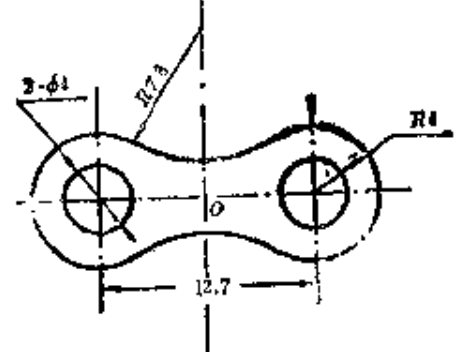
\includegraphics[width=5.5cm]{../pic/czjh2-ch7-subsec15-lx-02.png}
        \caption*{(第 2 题)}
    \end{minipage}
\end{figure}

% \begin{figure}[htbp] %
%     \centering
%     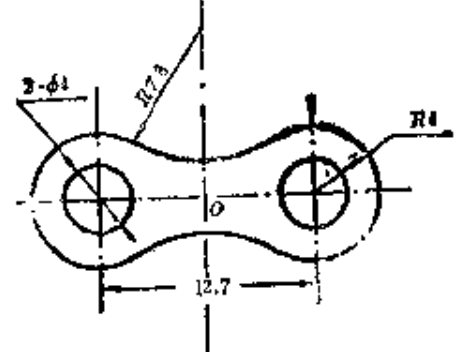
\includegraphics[width=5.5cm]{../pic/czjh2-ch7-subsec15-lx-02.png}
%     \caption*{(第 2 题)}
% \end{figure}

四条弧连接组成的图形就是椭圆的近似图形。

\begin{lianxi}

\xiaoti{说明近似椭圆的四条弧为什么是连接的。}

\xiaoti{按 $4:1$ 的比例尺,作出对应的图样。} % 原题为 “作出下面的图样”,因为排版的原因,将题目调整了一下
% 图片的代码原本应该放在这里,但由于分页时,将图片放在下一页。
% 而此后紧跟着 "习题 二十六",为了避免将此图误以为是“习题 二十六”中的图,
% 所以,将代码上移。

\end{lianxi}

